%*****************************************
\chapter{Lambdapi}\label{ch:intro-lambdapi}
%*****************************************

\section{The \texorpdfstring{\lp } - calculus modulo}

The \lp-calculus modulo rewriting (\lpm)  extends the Edinburgh Logical Framework (LF) \cite{lf} by allowing user-defined rewrite rules at both the term and type levels.
In this framework, all terms and types are identified modulo the congruence relation generated by standard $\beta$-reduction together with the specified rewrite rules.
{\lpm} is implemented in the Lambdapi proof language \cite{lambdapi}. Lambdapi, a successor of the Dedukti proof language \cite{Dedukti-ref, Dedukti-ref2}, is an implementation of {\lpm}; Lambdapi differs primarily by offering an integrated proof tactic language.
However, it can still import and export Dedukti theories to maintain compatibility. Lambdapi, similarly to Dedukti, is designed to facilitate the exchange of proofs between systems.
Lambdapi/Dedukti was used to translate \cite{thire:tel-03224039} the Matita arithmetic library to several systems, including Coq and PVS, export \cite{blanqui:hal-04613926} the HOL Light standard library to Coq,
and verify Event-B proofs \cite{eventb2lp}.

% \section{An assembly for proof assistant}

\begin{figure}[t]
    \centering
    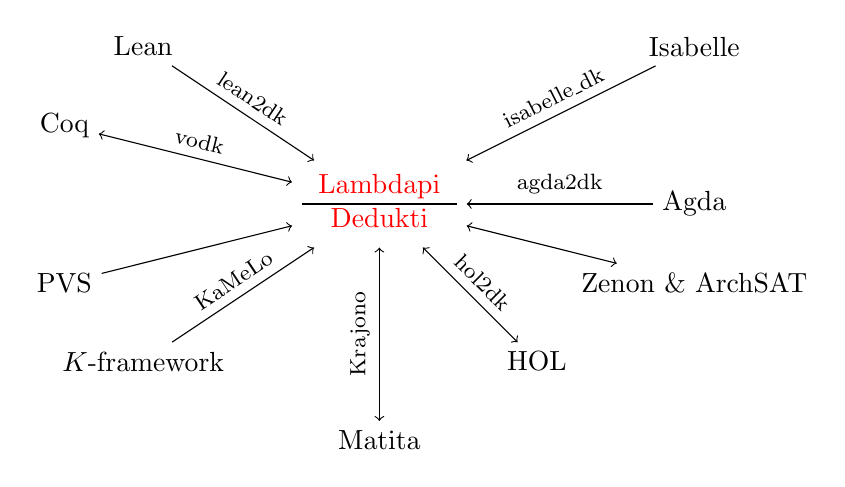
\begin{tikzpicture}
      \path (0,0) node (lp) {\begin{tabular}{c}
        \textcolor{red}{Lambdapi} \\
        \hline
        \textcolor{red}{Dedukti}
      \end{tabular}}
            (-4,1) node (coq) {Coq}
            (-3,2) node (lean) {Lean}
            % (0,2) node [draw, dashed, purple] (smt) {\color{purple}\textbf{SMT}}
            (4,2) node (isa) {Isabelle}
            (4,0) node (agda) {Agda}
            (-3,-2) node (k) {$\mathbb{K}$-framework}
            (0,-3) node (mat) {Matita}
            (2,-2) node (hol) {HOL}
            (-4,-1) node (pvs) {PVS}
            (4,-1) node (ze) {Zenon \& ArchSAT}
            ;
      % \draw[->,red, thick] (smt) -- (lp) node[midway,sloped,above]
      % {\footnotesize{Carcara}};
      \draw[->] (lean) -- (lp) node[midway,sloped,above] {\footnotesize{lean2dk}};
      \draw[->] (isa) -- (lp) node[midway,sloped,above] {\footnotesize{isabelle\_dk}};
      \draw[->] (agda) -- (lp) node[midway,sloped,above] {\footnotesize{agda2dk}};
      \draw[<->] (ze) -- (lp) node[midway,sloped,above] {};
      \draw[<->] (hol) -- (lp) node[midway,sloped,above] {\footnotesize{hol2dk}};
      \draw[<->] (mat) -- (lp) node[midway,sloped,above] {\footnotesize{Krajono}};
      \draw[->] (pvs) -- (lp);
      \draw[->] (k) -- (lp) node[midway,sloped,above] {\footnotesize{KaMeLo}};
      \draw[<->] (coq) -- (lp)  node[midway,sloped,above] {\footnotesize{vodk}};
    \end{tikzpicture}
    \caption{Lambdapi, an assembly language for proof systems.}
    \label{fig:interop}
\end{figure}

\section{Signature rules}

We start by defining the basic elements of the \lpm{} calculus and giving their syntax.
The terms of the \lp-calculus modulo are the same as in \lp-calculus (LF).
The Terms of \lpm{} are divided into three levels: Objects (denoted by $M$ and $N$), Types (denoted by $A$ and $B$), and Kinds (denoted by $K$).
The syntax of \lpm{} is given by the following grammar:


\begin{flalign*}
&\text{Objects}  & M, N  &::= c \pipe x \pipe \lambda\,x : A, M \mathrel{|} M~N &\\
&\text{Types}   & A,B &::= a \pipe \Pi\,x:A, B \pipe A~M &\\
&\text{Kinds} & K & ::= \type \pipe \Pi\,x:A, K &\\
&\text{Terms} & t,u & ::= M \pipe A \pipe K \pipe \kind  &
\end{flalign*}

where $c$ and $a$ are constants, and $x$ is a variable  (ranging over disjoint sets).
Dependent products  $\Pi\,x : A,\,B$ (respectively $\Pi\,x : A,\,K$) are simply written $A \rightarrow B$ when $x$ does not occur in $B$ (respectively $K$), $\lambda\,x : A,\,M$ is an abstraction, and  $M~N$ (respectively $A~M$) is an application.

\begin{definition}[Substitutions]
A substitution $\sigma$ is a function written \([ x_1 \leftarrow N_1, \dots, x_n \leftarrow N_n]\), from the variables to the terms with a finite domain.
We write $t\sigma$ the term $t$ where the variables are replaced by their image by $\sigma$.
\end{definition}

Contexts $\Gamma$ are finite sequences used to specify the type of the free variables.
Signatures (denoted $\Sigma$) serve as the \emph{global context} and are used to declare the constants and rewrite rules considered by the users.

\begin{flalign*}
&\text{Contexts}  & \Gamma  &::= \langle\rangle \pipe \Gamma,x: A &\\
&\text{Signature} & \Sigma &::= \langle\rangle \pipe \Sigma, c: A \pipe \Sigma, a: K \pipe \Sigma, M \re N  &\\
&                 &        &\qquad \pipe \Sigma,A \re B \pipe c \is A: M &
\end{flalign*}

A \emph{signature} \index{$\Sigma$} is a finite sequence of \emph{assumptions} $c : A$ (respectively $a : K$), indicating that constant $c$ is of type $C$ (respectively kind $K$), \emph{definitions} $c := A : M$, indicating that $c$ has the value $M$ and type $A$.
We write $\langle\rangle$ when contexts or signatures are empty. Rewrite rules are pairs $M \re N$ (respectively $A \re B$), where the head symbol of $M$ (respectively $A$) is a constant
and where free variables of $N$ (respectively $B$) occur in M (respectively $A$).
Rules must also preserve typing (subject-reduction property) as detailed in \cref{sect:lambdapi-typing}, that is, if an instance of a left-hand side has some type, then the corresponding instance of the right-hand side should have the same type. 
% The rewrite rules must preserve typing, i.e., whenever $\Gamma \vdash_\Sigma t\sigma: A$ with any substitution $\sigma$, and $t \longrightarrow_{\beta\Sigma} v$ then $\Gamma \vdash_\Sigma v\sigma: A$, as explained in \cref{sect:lambdapi-typing}.
A symbol with a definition cannot appear at the head of $M$ (or $A$) in a rewrite rule.

\begin{definition}[Delta reduction]
Let $\Sigma$ be a signature containing constant definitions of the form 
$c \coloneqq t$. 
We write
\[
c \;\;\rightarrow_\delta\;\; t
\]
to denote \emph{delta reduction}, that is, the replacement of the constant 
$c$ by its defining term $t$.
\end{definition}

In Lambdapi, delta reduction is applied implicitly during computation.
This means that whenever a defined constant appears in a term, it is automatically unfolded to its definition without requiring an explicit reduction step.


\begin{example}
Suppose the context contains the definition
\[
\mathsf{plus\_one} \coloneqq \lambda n.\, n + 1.
\]
Then we have the delta reduction
\[
\mathsf{plus\_one}\;2 \;\;\rightarrow_\delta\;\; (\lambda n.\, n + 1)\;2
\;\;\rightarrow_\beta\;\; 2 + 1.
\]
\end{example}



\section{Rewriting}
\label{sect:lambdapi-rw}

In the \lpm-calculus we distinguish two kinds of rewriting.

\subsection{\texorpdfstring{$\beta$}{}-reduction}

The first kind of rewriting is $\beta$-reduction, which is defined as usual.

\begin{definition}[$\beta$-reduction] The $\beta$-reduction relation $\longrightarrow_\beta$ is the smallest relation on terms containing
\( (\lambda x:A, u)v \longrightarrow_\beta u[x \leftarrow v] \) for any $A$, $u$, $v$ with type $A$ and closed by subterm reduction,
meaning that if $t \longrightarrow_\beta t'$, then the reduction also holds inside any larger term context containing $t$.
\end{definition}

\begin{notation}
We write $\longrightarrow^*_\beta$ for the reflexive and transitive closure of $\longrightarrow_\beta$ and $\equiv_\beta$ for the congruence generated by $\longrightarrow_\beta$.
\end{notation}

\subsection{\texorpdfstring{$\Sigma$}{}-reduction}

The second kind of rewriting is $\Sigma$-reduction, the relation generated by the rewrite rules of a signature $\Sigma$.

\begin{definition}[$\Sigma$-reduction]
Let $\Sigma$ be a global context. The  $\Sigma$-reduction relation $\longrightarrow_\Sigma$ is the smallest relation on terms containing $u \longrightarrow_\Sigma v$
for each rule $u \re v \in \Sigma$ and closed by substitution and subterm reduction.
\end{definition}

\begin{notation}
We write:

\begin{itemize}
\item $\longrightarrow^*_{\Sigma}$ the reflexive and transitive closure of $\longrightarrow_\Sigma$;
\item $\equiv_\Sigma$ the congruence generated by $\longrightarrow_{\Sigma}$;
\item $\longrightarrow_{\beta\Sigma}$ for $\longrightarrow_{\beta} \cup \longrightarrow_{\Sigma}$;
\item $\longrightarrow^*_{\beta\Sigma}$ the reflexive and transitive closure of $\longrightarrow_{\beta\Sigma}$;
\item $\equivL$ for the equivalence relation generated by $\longrightarrow_{\beta\Sigma}$.
\end{itemize}
\end{notation}

Lambdapi implements untyped rewriting because it will be inefficient to check the well-typedness of the substitution at each reduction step.

\begin{definition}[Linearity]
We also define the following properties:
\begin{itemize}
\item A term is linear if no variable occurs twice in it;
\item A rewrite rule $M \re N$ is left-linear if $M$ is linear.
\end{itemize}
\end{definition}

\begin{example}[Non-linear rule]
The rule $\kw{C}~x~x~y\re u$ is non-left linear because the variable $x$ occurs twice on the left of the arrow.
\end{example}

\section{Typing system}
\label{sect:lambdapi-typing}

We now give the typing rules of the \lpm{}-calculus in \cref{fig:lp-typing-rules}.
A Lambdapi typing judgment $\Gamma \vdash_\Sigma t : A$ asserts that term $t$ has type $A$ in the context $\Gamma$ and the signature $\Sigma$.


\begin{definition}[Well-Typed Term]
We say that a term $t$ has a type $A$ in a signature $\Sigma$ and a context $\Gamma$ if the judgment $\Gamma \vdash_\Sigma t: A$ is
derivable by the inference rules of \cref{fig:lp-typing-rules}. We say that a term is well-typed if such an $A$ exists.
\end{definition}

\begin{definition}[Well-Formed Local Context]
A local context $\Gamma$ is well-formed with respect to a global context $\Sigma$ if the judgment $\vdash_\Sigma \Gamma$ is derivable by the inference rules of \cref{fig:lp-typing-rules}.
\end{definition}


\begin{figure}
  \textbf{Contexts:}
  \[
    \begin{prooftree}
      \infer0[(Empty)]{ \vdash_\Sigma \langle\,\rangle  }
    \end{prooftree}
    \qquad
    \begin{prooftree}
      \hypo{ \vdash_\Sigma \Gamma }
      \hypo{ \Gamma \vdash_\Sigma A : s }
      \infer2[(Decl) $x \notin \Gamma$]{ \vdash_\Sigma \Gamma, x : A  }
    \end{prooftree}
  \]
  \textbf{Terms:}
  \medskip
  \begin{center}
    \begin{prooftree}
    \hypo{ \vdash_\Sigma \Gamma }
    \hypo{\Gamma \vdash_\Sigma A : s}
    \infer2[(Const)]{ \Gamma \vdash_\Sigma c : A }
    \end{prooftree}
  \end{center}
  \medskip
  \[
    \begin{prooftree}
      \hypo{ \vdash_\Sigma \Gamma }
      \infer1[(Sort)]{ \Gamma \vdash_\Sigma \type : \kind }
    \end{prooftree}
    \qquad
    \begin{prooftree}
      \hypo{ \vdash_\Sigma \Gamma }
      \infer1[(Var) $x : A \in \Gamma$]{ \Gamma \vdash_\Sigma x : A }
    \end{prooftree}
  \]

  \medskip

  \begin{center}
    \begin{prooftree}
      \hypo{ \Gamma \vdash_\Sigma  t : A }
      \infer1[(Delta)]{ \Gamma \vdash_\Sigma c : A \is t }
    \end{prooftree}
  \end{center}

  \medskip

  \begin{center}
    \begin{prooftree}
    \hypo{\Gamma, \vdash_\Sigma A : \type }
    \hypo{\Gamma, x: A \vdash_\Sigma B: s}
    \hypo{\Gamma, x : A \vdash_\Sigma t: B}
    \infer3[(Abs)]{ \Gamma \vdash_\Sigma \lambda x: A, t : \Pi x : A, B }
    \end{prooftree}
  \end{center}

  \begin{center}
    \begin{prooftree}
      \hypo{ \Gamma \vdash_\Sigma A : \type }
      \hypo{ \Gamma, x : A \vdash_\Sigma B : s }
      \infer2[(Prod)]{ \Gamma \vdash_\Sigma \Pi x : A, B : s }
    \end{prooftree}
    \quad
  \end{center}

  \medskip

  \begin{center}
    \begin{prooftree}
      \hypo{ \Gamma \vdash t : \Pi x : A, B }
      \hypo{ \Gamma \vdash  u : A }
      \infer2[(App)]{ \Gamma \vdash_\Sigma t~u : B[u \leftarrow x] }
    \end{prooftree}
  \end{center}

  \medskip

  \begin{center}
  \begin{prooftree}
  \hypo{\Gamma, \vdash_\Sigma B: u}
  \hypo{\Gamma \vdash_\Sigma t: A}
  \hypo{A \textcolor{red}{\equiv_{\beta\Sigma}} B}
  \infer3[(Conv)]{ \Gamma \vdash_\Sigma t: B }
  \end{prooftree}
  \end{center}
  \caption{Typing rules of \lpm}
  \label{fig:lp-typing-rules}
  \end{figure}

\begin{remark}
The typing rules shown in \cref{fig:lp-typing-rules} are similar to those of  \lp{}-calculus \cite[\S 2]{lf}, except for the additional rule (Conv) that identifies types modulo $\equivL$ instead of just modulo $\equiv_\beta$.
\end{remark}


The main difference between the \lp-calculus and the \lpm-calculus is the presence of the rewrite rules in global contexts.
We need to take this into account when typing global contexts. A key feature of any type system is the preservation of typing by reduction: the subject reduction property.

\begin{definition}[Subject Reduction]
Let $\longrightarrow_r$ be a binary relation on terms.
We say that a global context $\Sigma$ satisfies the \emph{subject reduction} property for $\longrightarrow_r$ if the following holds:
for any well-formed local context $\Gamma$ with $\Sigma$, for any terms $t_1$ and $t_2$ such that $t_1 \longrightarrow_r t_2$, and for any term $T$,
if $\Sigma, \Gamma \vdash t_1 : T$ then $\Sigma, \Gamma \vdash t_2 : T$.
\end{definition}

In the \lpm calculus, allowing arbitrary rewrite rules in the context could breaks properties such as subject reduction for relation $\longrightarrow_{\beta\Sigma}$.
Lambdapi requires user rules in $\longrightarrow_{\beta\Sigma}$ for the encoded theories to be \emph{confluent} (\cref{def:confluence-rew}) and typing-preserving, even if it does not automatically check that confluence holds.

\begin{definition}[Confluent $\longrightarrow_{\beta\Sigma}$]\label{def:confluence-rew}
The relation $\longrightarrow_{\beta\Sigma}$ must be confluent, i.e., whenever $t \longrightarrow_{\beta\Sigma}^* v_1$ and $t \longrightarrow_{\beta\Sigma}^* v_2$, there exists a term $w$ such that $v_1 \longrightarrow_{\beta\Sigma}^* w$ and $v_2 \longrightarrow_{\beta\Sigma}^* w$.

\begin{center}
\begin{tikzpicture}
\node (a) at (0,2) {$t$};
\node (b) at (-2,0) {$v_1$};
\node (c) at (2,0) {$v_2$};
\node (d) at (0,-2) {$w$};

\draw[->] (a) -- (b) node[midway, above left] {$*$};
\draw[->] (a) -- (c) node[midway, above right] {$*$};
\draw[->, dashed] (b) -- (d) node[midway, below left] {$*$};
\draw[->, dashed] (c) -- (d) node[midway, below right] {$*$};

\node at (0,-3) {\textit{Confluence Property}};
\end{tikzpicture}
\end{center}
\end{definition}

In other words, confluence is a property of rewriting systems, describing the condition where terms in such a system can be rewritten in more than one way to yield the same result.

\begin{remark}
External tools, such as CSI \cite{CSI}, can be used to verify the confluence of a set of rewriting rules with a Signature.
Lambdapi can export its rules and the signature $\Sigma$ in a format accepted by CSI.
\end{remark}

One approach to prove the confluence property that we will now describe is to check that the critical pairs (\cref{def:critical-pair}) of the rewrite rules in $\Sigma$ are joinable.

\begin{definition}[Position and Subterm]
Let $t$ be a term. We denote $Post(t)$ the set of positions in $t$ that is a sequence of integers and the subterm $t_{| p}$ of $t$
at position $p \in Post(t)$ are defined inductively as follows:
\begin{itemize}
  \item if $t$ is a variable, then $Post(t) = \{ \epsilon \}$ and $t_{| \epsilon} = t$;
  \item if $t = f~t_1 \dots t_n$, then
    \begin{itemize}
      \item[] \( Post(t) = \{ \epsilon \} \cup \{1.q \pipe q \in Post(t_1)\} \cup \dots \cup \{n.q \pipe q \in Post(n_1)\} \),
      \item[] and \( t_{| \epsilon} = t \),
      \item[] and \( t_{| i.q} = t_{i|q} \)
    \end{itemize}
\end{itemize}
\end{definition}

\begin{definition}[Critical pair]\label{def:critical-pair}
Let $l_i \re r_i$ (for $i = 1, 2$) be two rewrite rules. Suppose that they do not share any variable (variables can be renamed if needed).
If there exists $p \in Post(l_1)$ such that $l_{1 | p}$ is not a variable and $\sigma$ a unifier of $l_{1 | p}, l_2$ then
we have the following reduction $l_1 \sigma \re (l_1\sigma)[l_2\sigma]_p$. We say that the pair $((l_1\sigma)[l_2\sigma]_p, r_1\sigma)$ is a
critical pair and that the two rewrite rules overlap.
\begin{center}
\begin{tikzpicture}
% Top term showing the overlap
\node (top) at (0,3) {$l_1\sigma$};

% The two reductions from the overlapping term
\node (left) at (-3,1) {$(l_1\sigma)[r_2\sigma]_p$};
\node (right) at (3,1) {$r_1\sigma$};

% Arrows showing the reductions
\draw[->] (top) -- (left) node[midway, above left] {$l_2 \to r_2$ at $p$};
\draw[->] (top) -- (right) node[midway, above right] {$l_1 \to r_1$};

\node (bot) at (0,-1) {?};

% Dashed arrows showing potential confluence
\draw[->, dashed] (left) -- (bot);
\draw[->, dashed] (right) -- (bot);

% \node at (0,-2.3) {\textit{Must be joinable for confluence}};
\end{tikzpicture}
\end{center}
\end{definition}

\begin{definition}[Joinable]
Two term $x, y \in \Sigma$ are \emph{joinable} (written $x \downarrow y$), if there exists $z$ such that $x \re^* z$ and $y \re^* z$.
\end{definition}

To guarantee confluence of Lambdapi's rewrite system with user-defined rules we leverage local confluence. 
This property acts as a stepping stone toward full confluence via Newman's lemma (\cref{lem:newman}), provided the system is also terminating.

\begin{definition}[Local confluence]
A constant $a \in \Sigma$ is \emph{locally confluent} if for all constants $b,c \in \Sigma$ with the rewrite rules $a \re b$ and $a \re b$
we have $b \downarrow c$. The $\Sigma$ is locally confluent if all its elements are locally confluent.
\end{definition}

\begin{theorem}[Critical Pair Theorem]\label{thm:cp}
The set of rewrite rules $R$ over the signature $\Sigma$ (and its set of variables $\cal{V}$) is locally confluent if and only if its critical pairs are joinable.
\end{theorem}


\begin{lemma}[Newman’s Lemma]\label{lem:newman}
If the set of rewriting of a signature $\Sigma$ is \emph{terminating} (i.e., there is no infinite sequence
$x_0 \re x_1 \re x_2 \re \cdots$) and \emph{locally confluent} (i.e., for all $s,u,v \in \Sigma$, if $s \re u$ and $s \re v$ then there exists
$c \in \Sigma$ such that $u \re^{*} c$ and $v \re^{*} c$), then it is confluent (i.e., for all $s,u,v \in \Sigma$, if $s \re^{*} u$ and
$s \re^{*} v$ then there exists $w \in \Sigma$ such that $u \re^{*} w$ and $v \re^{*} w$).
\end{lemma}

\begin{remark}
Similar to Confluence, Lambdapi does not verify that a set of rules terminates.
However, external tools such as AProVe \cite{aprove} can be used to check the termination of a set of rewriting rules with a signature.
Lambdapi can export its definitions and Signature into a format accepted by the tool AProVe.
\end{remark}

Combining \cref{thm:cp} with \cref{lem:newman} we get the following result:

\begin{corollary}
The set of rewrite rules $R$ over the signature $\Sigma$ is confluent if and only if its critical pairs are joinable.
\end{corollary}

A complete proof of subjection reduction for $\longrightarrow_\beta$ and $\longrightarrow_\Sigma$ can be found in \cite[\S 2.6.4]{Dedukti-ref2}.

\section{Prelude}
\label{sec:prelude-lp}

The Lambdapi standard library includes the following definitions, which we will reuse and contribute to enrich.

\begin{definition}[Prelude Encoding]
\label{def:defuniv}
The signature $\Sigma$ of our encoding contains the following definitions and rewrite rules that we use to encode Alethe proofs:
\begin{align*}
&\set\index{\set}: \type & &\prop\index{\prop}: \type \\
&\index{\el{}} \el{}: \set \rightarrow \type  & &\index{\prf}\prf{} : \prop \rightarrow \type \\
&\mathop{\leadsto}\index{$\leadsto$}: \set \rightarrow \set \rightarrow \set \quad \text{(infix)} & &o: \set \\
&\el\,(x \leadsto y) \hookrightarrow (\el\,x \rightarrow \el\,y) & &\el\,o\index{o}  \hookrightarrow \prop \\
& {=} : \Pi [a : \set], \el\, a \ra \el\, a \ra \prop & & \text{(infix)}
\end{align*}
\end{definition}

The notions of term, proposition, and proof are not primitive in \lpm.
We first define a notion analogous to the predicate logic notion of term, to express the objects the theory speaks about, such as the natural numbers.
The constants \set{} and \prop{} in \cref{def:defuniv} are type universes ``à la Tarski'' \cite[\S Universes]{intuitype} in \lpm.
The type \set{} will be used to represent the universe of \textit{small types}, i.e.\ a subclass of types for which we can define equality.
Since elements of type \set{} are not types themselves,
we also introduce a function $\el: \set \rightarrow \type$ that embeds the terms of type \set{} into terms of type \type.
Equality (=) over small types is parameterized over types $\el\,a$ for the type parameter $a : \set{}$.

Just as \lpm{} does not contain a primitive notion for expressing the objects of the theory, it does not contain a primitive notion of proposition.
The constant \prop{} represents the universe of propositions. Predicate symbols are represented as constants of type $\set{} \ra \dots \ra \prop$ .
Similar to \set{}, elements of type \prop{} are not types themselves; they are mapped to types by the function $\prf{}: \prop \rightarrow \type$.
Drawing an analogy with the Curry-de-Brujin-Howard isomorphism \cite{curryhoward}, this function embeds propositions into types by mapping each proposition $A$ to the type $\prf\,A$, which represents its proofs.
However, the analogy is only partial in two important ways. First, the propositions themselves are not the types of their proofs: if $t$ is a proof of $A$, then it does not have the type $A$,
but the type $\prf\,A$. Second, the embedding is not surjective—meaning not all types correspond to proofs. For instance, neither \set{} nor \prop{} is itself a type of proof.

Consequently, a \emph{step} in an Alethe proof trace is represented as an inhabitant of type $\prf{}\,p$, for a suitable proposition $p$.

\begin{example}[Multiplication group]\label{ex:group}
The encoding of the multiplication group with a multiplication symbol $\times$, an inverse operation $inv$ and a neutral element $1$.
\[
\begin{array}{lll}
\iota : \type & \times : \iota \to \iota \to \iota & \text{inv} : \iota \to \iota \\
1 : \iota & x \times 1 \re x & x \times (\text{inv } x) \re 1 \\
\text{inv } (\text{inv } x) \re x & 1 \times x \re x & (\text{inv } x) \times x \re 1 \\
\text{inv } 1 \re 1 & (x \times y) \times z \re x \times (y \times z) & \\
\end{array}
\]
\end{example}

\begin{lstlisting}[language=Lambdapi,caption={Concrete syntax of \cref{ex:group}}, label={lst:concrete-syntax}]
symbol ι : TYPE;
symbol × : ι → ι → ι;
symbol 1 : ι;
symbol inv : ι → ι;

rule $x × 1 ↪ $x;
rule 1 × $x ↪ $x;
rule ($x × $y) × $z ↪ $x × ($y × $z);
rule $x × (inv $x) ↪ 1;
rule (inv $x) × $x ↪ 1;
rule inv 1 ↪ 1;
rule inv (inv $x) ↪ $x;
\end{lstlisting}

The \cref{lst:concrete-syntax} above shows the concrete syntax for the group specification. In Lambdapi's concrete syntax, constants are declared using the \lpinline{symbol} keyword,
while variables in rewrite rules are prefixed with \kw{\$} to distinguish them from constants during pattern matching.


\section{Constructive connectives, quantifiers}
\label{ssec:encoding-prop}

In our framework, we adopt the standard set of logical operators and axioms from intuitionistic logic.

\begin{definition}[Constructive connectives, quantifiers]
\begin{align}
& \top : \prop \\
& \bot : \prop \\
& \land : \prop \ra \prop \ra \prop \qquad \text{(written infix)} \\
& \lor : \prop \ra \prop \ra \prop \qquad \text{(written infix)} \\
& \Rightarrow : \prop \ra \prop \ra \prop \qquad \text{(written infix)} \\
&  \prf\,(a \Rightarrow\,b) \re \prf\, a \ra \prf\,\,b \label{eq:imp}\\
& \neg a \is a \Rightarrow \bot \\
% & \mathop{\mathrm{xor}}~a~b \is (\neg a \land b) \lor (a \land \neg b) \\
& \forall : \Pi {[a: \set]}, (\el\, a \ra \prop) \ra \prop \label{eq:forall}\\
& \prf{}(\forall\,p) \re \Pi\, x, \prf{(p~x)}\\
& \exists : \Pi\, {[a: \set]}, (\el\, a \ra \prop) \ra \prop
\end{align}
\end{definition}

According to the Curry-de Bruijn-Howard correspondence, a proof of $A \Rightarrow B$ should have the type $\prf\,(A \Rightarrow B)$.
However, such a proof actually has type $\prf\,A \ra \prf\,B$. This means that the types $\prf\,(A \Rightarrow B)$ and $\prf\,A \ra \prf\,B$ must be identified.
To achieve this, we introduce the rewriting rule \cref{eq:imp}, allowing $\prf\,(A \Rightarrow B)$ to be rewritten as $\prf\,A \ra \prf\,B$.

We cannot assign the type $\Pi\,X: \type, (X \ra \prop) \ra \prop$ to the universal quantifier, because in \lpm{} there is no mechanism for quantifying over variables of type \type.
Instead, we assign the type $\Pi\,x:\set{},(\el\,x \ra \prop) \ra \prop$ to the generic universal quantifier $(\forall)$ \cref{eq:forall}.
Furthermore, the previously defined term $o: Set$, together with the rewrite rule $\el\,o\index{o} \hookrightarrow \prop$ enables quantification over propositions, rendering the universal quantifier impredicative.

\begin{example}[quantification over $\prop$ with $o$]
The eliminator for the bottom ($\bot$) can be formalized as:
\[ \bot_e : \prf\,(\bot \Rightarrow \forall (p: \el\,o), p) \]
\end{example}

\begin{example}[Product type]\label{def-product}
The product type, which pairs together values from two types, is constructed as follows:
\begin{align*}
&\textbf{Non dependent product type:} \\
&\quad \times : \text{Set} \to \text{Set} \to \text{Set} \quad \textit{(written infix)} \\
&\textbf{Pairing symbol:} \\
&(\mathbin{‚}) [a~b] : \el a \ra \el b \ra \el (a \times b)\\[1em]
&\textbf{Projections (written postfix):}  \\
&\quad {}_1 : \el\, (a \times b) \ra \el\, a \quad \text{with rewrite rule } (x \mathbin{‚} \_)_1 \re x \\
&\quad {}_2 : \el\, (a \times b) \ra \el\, b \quad \text{with rewrite rule } (\_ \mathbin{‚} y)_2 \re y
\end{align*}
The pairing constructor is denoted by $(‚)$ (a comma-like symbol), which takes two terms $x : \el\,a$ and $y : \el\, b$ and produces a term $x \mathbin{‚} y : \el (a \times b)$.
Two projection symbols ${\_}_1$ and ${\_}_2$ extract the first and second components of a pair, respectively.
\end{example}

\subsection{Inductive data structure}

To illustrate how inductive types are expressed in Lambdapi, we present below some data structures.
While these examples are is primarily intended to demonstrate the syntax and capabilities of the system, some of these structures will later be employed in our encoding in \cref{ch:encoding}.
Lambdapi extends the \lpm-calculus modulo by providing partial support for inductive types.
An inductive type is declared by specifying its name, followed by a list of constructors $C_i$, each describing one possible way of building an element of the type.
The general form is:

\begin{align*}
&(a_1 : A_1 \dots a_1 : A_n)~T : I_1 \ra \dots I_n \ra \type\\
&|~C_1 : \dots : T \dots\\
&|~C_2 : \dots : T \dots\\
&\vdots
\end{align*}

The (possibly empty) set $(a_1 : A_1 \dots a_n : A_n)$ represents the parameters, while the (possibly empty) set $I_1, \dots, I_n$ represents the indices.
This support is described as partial because Lambdapi currently does not enforce the positivity constraint on inductive definitions \cite[\S 2.2]{inductive-type}.
From any inductive type declaration, Lambdapi automatically derives the corresponding induction principle along with its associated inference rules.
A current limitation exists forcing inductive type to be of kind $\type$, so for example it is not possible to create inductive predicates ($\prop$).


\begin{definition}[Natural]\label{def-nat}
The Peano numbers are defined as:
\begin{align*}
&\N: \type \\
&|~0 : \N \\
&|~+\!\!1: \N \ra \N \quad \text{(written postfix)} \\[1em]
& \kw{nat}~: \set \\
&  \el~\kw{nat} \re \N
\end{align*}
\end{definition}

We make use of Lambdapi's \lstinline[language=Lambdapi,basicstyle=\ttfamily\footnotesize]|builtin| mechanism to enable decimal notation for numeric values, allowing us to write, e.g., $2$ instead of $((0 +\!\!1) +\!\!1)$.

\begin{definition}[Boolean]\label{def-bool}
The booleans are defined as:
\begin{align*}
&\B: \type \\
&| \true : \B \\
&| \false : \B \\[1em]
& \kw{bool}~: \set \\
&  \el~\kw{bool} \re \B
\end{align*}
\end{definition}

\begin{definition}[List]\label{def:list}
The inductive type for lists is defined as follows:
\begin{align*}
&(a: \set)~ \bb{L}: \type \\
&|~\Box : \bb{L}~a \\
&|~\mathrel{::}~: \el  a \ra \bb{L}~a \ra \bb{L}~a \quad \text{(written infix)} \\[1em]
& \kw{list}~: \set \ra \set \\
&  \el~(\kw{list}~a) \re \bb{L}~a
\end{align*}
where the constructor $\Box$ represents the empty list and $\mathrel{::}$ represents the cons operation that prepends an element to a list.
For example, the list containing elements $x$, $y$, and $z$ (in that order) is written as $x \mathrel{::} y \mathrel{::} z \mathrel{::} \Box$.
\end{definition}


\begin{definition}[Dependent pair]\label{dep-pair-def}
The type $\int$ parameterized by a predicate $p$ on a type $\el\,a$, represents a dependent pair consisting of an element $x : \el\,a$ and a proof that $p~x$ holds.

\begin{align*}
&\int : \forall a : \set{}, (\el{}~a \ra \prop): \type \\
&|~exist : \Pi (x :\el{}\,a), \prf (p~x) \ra \int~p \\
&\\
& int~[a: \set{}]: (\el{}~a \ra \prop) \ra \set{} \\
& \el{}~int~p \re \int~p \\
&\\
& \textcolor{red}{s_1}~[a: \set{}] [p:(\el{}~a \ra \prop)] (e: \int~a~p): \el{}~a \\
& (exist~x~\_)~\textcolor{red}{s_1} \re x\\
& s_2~[a: \set{}] [p:(\el{}~a \ra \prop)] (e: \int~a~p): \prf{}(p~(e~\textcolor{red}{s_1})) \\
& (exist~\_~p)~s_2 \re p\\
\end{align*}
The projections from this dependent pair are defined through the symbols $s_1$ and $s_2$, corresponding respectively to the first and second components of the pair.
The rewrite rule for $s_1$ extracts the value $x$ from a term of the form $\kw{exist}~x~\_$, while the rule for $s_2$ retrieves the proof that $(p~x)$ holds.
\end{definition}

\begin{definition}[Dependent vector]\label{def:dependent-vector}
The type \( \mathop{\mathrm{Vec}}\,a\,n \) of vectors of elements of $a$ of length $n$.
We define the constant \( \mathop{\mathrm{Vec}}\,a\,n \) inductively for \( n : \N \) as:
\begin{align*}
&(a: \set) \mathop{\mathrm{Vec}}: \N \ra \type \\
&|~\Box_\bb{V} : \mathop{\mathrm{Vec}} a \, 0 \\
&|~\cons_\bb{V}\,[n:\N]: \el\,a \ra \mathop{\mathrm{Vec}}\,a\,n \ra  \mathop{\mathrm{Vec}}\,a\,(n +1) \quad (\text{infix})\\
&\mathop{\mathrm{vector}}: \set \ra \N \ra \set \\
&\el~(\mathop{\mathrm{vector}}\,a\,n) \re \mathop{\mathrm{Vec}}\,a\,n
\end{align*}
\end{definition}

\section{Modifiers on symbols}

Lambdapi modifiers are keywords that precede a constant declaration to provide the system with additional information on its properties and behavior.
We will present the modifiers \lpinline{sequential} and \lpinline{associative commutative} that will be use in the contributions of this thesis.

\subsection{Sequential}

The modifier \lpinline{sequential} alters the pattern matching algorithm.
By default, the order of rule declarations is not taken into account.
This modifier tells Lambdapi to apply rules defining a sequential symbol in the order they have been declared.
However, this rule can break important properties such as confluence or \emph{stable by substitution}.

\begin{lemma}[Stability by substitution]\label{lem:stability}
Suppose we have a typing judgment
\[
  \Gamma, x : A \;\vdash\; t : B
\]
and also a derivation
\[
  \Gamma \;\vdash\; u : A ,
\]
then replacing $x$ by $u$ in $t$ preserves typing:
\[
  \Gamma \;\vdash\; t[x \leftarrow u] : B[x \leftarrow u] .
\]
\end{lemma}

\begin{example}
Consider the constant $\kw{eq}: \prop \ra \prop \ra \B$ defined \lpinline{sequential} and the following non-linear set of rewrites rules:
\[
    \kw{eq}~x~x \re \true\\
    \kw{eq}~x~y \re \false
\]
Then it is not stable by substitution given the following substitution $\vdash\kw{eq}[x \leftarrow y]$ which breaks \cref{lem:stability}.
\end{example}

\subsection{Associative commutative}

Lambdapi handles associative and commutative symbols via \lpinline{associative commutative}, normalizing terms to a canonical form using a built-in ordering (\cite{ACorigin}, \cite[\S 5]{univAC}).

\begin{definition}[builtin ordering relation]\label{def:builtin-order-relation}
Let $T$ be a type with constructors $\epsilon : T$, $\mathtt{C_1} : A \to T$, $\mathtt{C_2} : A \to B \to T$, and $\mathtt{C_n} : \mathcal{T}_1 \to \cdots \to \mathcal{T}_n \to T$ for some arbitrary types $A, B, \mathcal{T}_1, \ldots, \mathcal{T}_n$ representing constructors of different finite arities.

The $\leq$ builtin total order on $T$-terms is defined as follows. Terms are ordered such that
\[
  \epsilon < \mathtt{C_1}(a) \leq \mathtt{C_1}(a') < \mathtt{C_2}(c, b) < \mathtt{C_n}(t_1, \ldots, t_n)
\]
for any terms $a \leq a'$ of appropriate types, any $c : A$, and any $b : B$.

\begin{itemize}
\item For $\mathtt{C_1}$ constructor terms, $\mathtt{C_1}(a_1) \leq \mathtt{C_1}(a_2)$ if and only if $a_1 \leq a_2$.

  \item For $\mathtt{C_2}$ constructor terms, $\mathtt{C_2}(c_1, b_1) \leq \mathtt{C_2}(c_2, b_2)$ if and only if either $c_1 < c_2$, or $c_1 = c_2$ and $b_1 \leq b_2$.

  \item For $\mathtt{C_n}$ constructor terms, $\mathtt{C_n}(t_1^{1}, \ldots, t_n^{1}) \leq \mathtt{C_n}(t_1^{2}, \ldots, t_n^{2})$ if and only if there exists some $k \in \{1, \ldots, n\}$ such that $t_i^{1} = t_i^{2}$ for all $i < k$ and $t_k^{1} < t_k^{2}$, or $t_i^{1} = t_i^{2}$ for all $i \in \{1, \ldots, n\}$.
\end{itemize}
\end{definition}

Now, consider a binary constructor $\oplus: T \to T \to T$ declared \lpinline{associative commutative}.
The transformation to canonical form implemented in Lambdapi ensures that $\oplus$ expressions such as:

\[
  (C_2~c_1~x_1) \oplus (C_1~k_1) \oplus (C_2~c_2~x_2) \oplus \dots \oplus (C_2~c_n~x_n)
\]

will be normalized following the builtin relation of \cref{def:builtin-order-relation}.

\begin{definition}
Let $\twoheadrightarrow^{AC}$ be the relation mapping every term $t$ to its unique AC-canonical form denoted $[t]$.
\end{definition}

\begin{definition}[AC equivalence]
Two terms $t$ and $u$ are AC-equivalent (written $t \simeq_{AC} u$) if and only if their AC-canonical forms are equal: $[t] = [u]$.
\end{definition}

\begin{example}
Consider the inductive type $\mathbb{M}$ below with 3 constructors of three different arities from $0$ to $2$, and the natural order on $\mathbb{N}$ terms:
\begin{align*}
&\bb{M}: \type \\
&|~\epsilon : \bb{M} \\
&|~P_1: \N \ra \bb{M} \\
&|~P_2 : \N \ra \N \ra \bb{M} \\
&|~ \oplus : \bb{M} \to \bb{M} \to \bb{M} \quad \text{(written infix)}
\end{align*}
We define $\oplus$ as \lpinline{associative commutative}. Therefore, the term
\[
  P_2(1,2) \oplus P_1(1) \oplus P_2(1,1) \oplus P_1(2) \oplus \epsilon
\]
is normalized to:
\[
  \epsilon \oplus P_1(1) \oplus P_1(2) \oplus P_2(1,1) \oplus P_2(1,2)
\]
\end{example}

\begin{remark}
The properties of \emph{local confluence} and \emph{termination} need to take AC-canonicalization into account to prove that they still hold.
\end{remark}


This chapter presented the \lp{}-calculus modulo rewriting as implemented in Lambdapi, highlighting how user rewrite rules at both the term and type levels extend LF.
We presented concrete data structures and the modifiers that will be used throughout the next chapters for our encoding.